\begin{center}

\includegraphics[width=0.60\textwidth]{imagenes/escudo.jpg}
\end{center}
%%%%%%%%%%%%%%%%%%%%
\vspace{0.5 cm}
\centerline{\large \sf UNIVERSIDAD NACIONAL DE COLOMBIA}
\centerline{\large \sf FACULTAD DE CIENCIAS}
\centerline{\large \sf OBSERVATORIO ASTRON\'OMICO NACIONAL} 
%%%%%%%%%%%%%%%%%%%
\vspace{1.0 cm}
{\fontencoding{T1}\fontfamily{phv}\fontseries{b}\fontshape{n}\fontsize{9}{9}\selectfont

\textcolor{1col}{\centerline{\large \sf Tesis para optar el t\'itulo de Magister en Ciencias - Astronom\'ia:}}}

\vspace{0.3 cm}

{\fontencoding{T1}\fontfamily{phv}\fontseries{b}\fontshape{n}\fontsize{9}{9}\selectfont

\textcolor{2col}{\centerline{\large \bf SOBRE LA ACELERACI\'ON ESTOC\'ASTICA DE ELECTRONES}
\vspace{1.4cm}
\centerline {\large \bf Y LA SISMICIDAD ASOCIADA A FULGURACIONES SOLARES}}}


%%%%%%%%%%%%%%%%%%%
%\vspace{1.5 cm}
\centerline{Bogot\'a - Colombia.}
\centerline{2013}
%%%%%%%%%%%%%%%%%%%%%%%%%%%%%%%%%%%%%%%%%%%%%%%%%%%%%%%%%%%%%%%%%%%%%%%%%%%%%%%%%%%%%%%%%%
\newpage
%%%%%%%%%%%%%%%%%%%%%%%%%%%%%%%%%%%%%%%%%%%%%
\clearpage
\begin{center}

\includegraphics[width=0.25\textwidth]{imagenes/un.jpg}
\end{center}
\centerline{\large \sf UNIVERSIDAD NACIONAL DE COLOMBIA}
\centerline{\large \sf FACULTAD DE CIENCIAS}
\centerline{\large \sf OBSERVATORIO ASTRON\'OMICO NACIONAL} 
%%%%%%%%%%%%%%%%%%%%%%%%%%%%%%%%%%%%%%%%%%%%%
\vspace{2.0 cm}
{\fontencoding{T1}\fontfamily{phv}\fontseries{b}\fontshape{n}\fontsize{9}{9}\selectfont

\textcolor{2col}{\centerline{\large \bf SOBRE LA ACELERACI\'ON ESTOC\'ASTICA DE ELECTRONES}
\vspace{2.0 cm}
\centerline {\large \bf Y LA SISMICIDAD ASOCIADA A FULGURACIONES SOLARES}}}
%%%%%%%%%%%%%%%%%%%%%%%%%%%%%%%%%%%%%%%%%%%%%

\centerline{\large{\bf Juan Camilo Buitrago-Casas}} 
\vspace{1.2 cm}
\centerline{\large {\it Director} :  Prof. Benjam\'in Calvo-Mozo}
\centerline{{\it Observatorio Astron\'omico Nacional, Bogot\'a-Colombia}}
\vspace{0.3 cm}
\centerline{\large {\it Asesor internacional} :  PhD. Juan Carlos Mart\'inez-Oliveros}
\centerline{{\it Space Sciences Laboratory, Berkeley University, California-USA}}
%%%%%%%%%%%%%%%%%%%%%%%%%%%%%%%%%%%%%%%%%%%%%
\vspace{0.5 cm}
\begin{center}
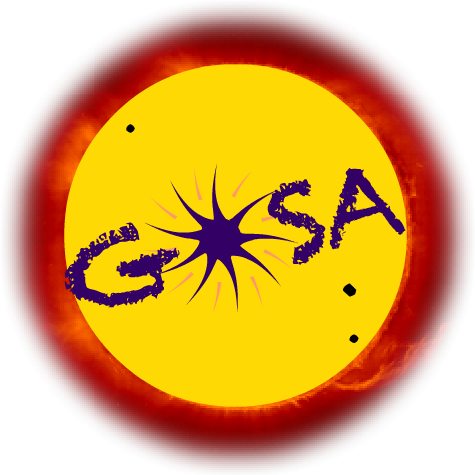
\includegraphics[width=0.17\textwidth]{imagenes/gosa.png}
\end{center}
\centerline{Bogot\'a-Colombia}
\centerline{2013}
%%%%%%%%%%%%%%%%%%%%%%%%%%%%%%%%%%%%%%%%%%%%%%%%%%%%%%%%%%%%%%%%%%%%%%%%%%%%%%%%%%%%%
\newpage
\centerline {\Large Sobre la aceleraci\'on estoc\'astica de electrones}
\centerline {\Large y la sismicidad asociada a fulguraciones solares.}
%%%%%%%%%%%%%%%%%%%%%%%%%%%%%%%%
\vspace{1.0 cm}
\centerline{Juan Camilo Buitrago-Casas} 
%%%%%%%%%%%%%%%%%%%%%%%%%%%%%%%%
\vspace{1.5 cm}
{\renewcommand{\baselinestretch}{1.5}
{\footnotesize
\begin{flushright}
\begin{minipage}[h]{9cm}
{ Trabajo de grado presentado al programa de Maestr\'ia en Ciencias Astronom\'ia de la Facultad de Ciencias de la Universidad Nacional de Colombia sede Bogot\'a como parte de los requisitos  de grado necesarios para obtener el t\'itulo de Magister en Ciencias: Astronom\'ia.\\\\
Director :  Prof. Benjam\'in Calvo-Mozo\\
Asesor internacional :  PhD. Juan Carlos Mart\'inez-Oliveros}
\end{minipage}
\end{flushright}}
%%%%%%%%%%%%%%%%%%%%%%%%%%%%%%%%%
\vspace{2.5 cm}
\centerline{\normalsize Banca Examinadora}
\begin{center}
\begin{tabular}{c}
\\\hline
Coordinaci\'on \'Area Curricular de la Maestr\'ia en Ciencias: Astronom\'ia\\
\end{tabular}
\end{center}
%%%%%%%%%%%%%%%%%%%%%%%%%%%%%%%%%
\vspace{1.0 cm}
\begin{center}
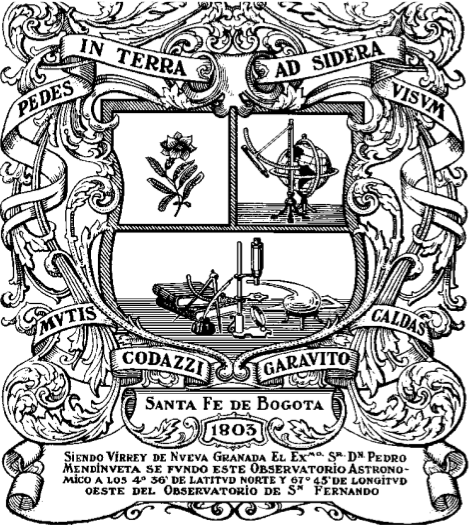
\includegraphics[width=0.35\textwidth]{imagenes/oan.png}
\end{center}

\renewcommand\contentsname{Contenido} 
\clearpage
\tableofcontents
\setcounter{page}{3}
\newpage
